\subsection{Out-of-cone radiation}\label{sec:preceloss}

%{\it (pmj comment Nov 5: I am not clear about the choice of title "Precision energy loss" for this section. We are aiming for high precision in Run 3/4 in many different observables related to energy loss and jet modification, of which the observables discussed in this section are a subset, covering limited phase space. But identifying the observables in the phase space described in this section as "precision" measurements implies that measurements that are not described here are in some sense less precise - both experimentally and in terms of theoretical interpretation - which I do not support. I don't think we will resolve these questions in this group, and suggest that a more neutral title be found for this subsection.)}

One of the classic observables to measure the out-of-cone radiation due to jet quenching is the jet nuclear modification factor $R_{\mathrm{AA}}$ defined as: 
  \begin{equation} 
  \RAA=\dfrac{ \left.\dfrac{1}{N_{\mathrm{evt}} }\dfrac{\mathrm{d}^{2} 
N_{\mathrm{jet}}}{\mathrm{d} \pT \mathrm{d} y} \right|_{\mathrm{cent}}
}
{
\left. \TAA \dfrac{\mathrm{d}^2 \sigma_{\mathrm{jet}}}{\mathrm{d} \pt \mathrm{d} y}\right|_{pp}
}\, ,
\label{eq:RAAjet}
\end{equation} 
where $N_{\mathrm{jet}}$ and $\sigma_{\mathrm{jet}}$ are the jet yield in Pb--Pb collisions and the jet production cross-section in pp collisions, 
respectively, both measured as a function of transverse momentum, \pT, and rapidity, $y$, and where $N_{\mathrm{evt}}$ is the total number of Pb--Pb collisions within a chosen centrality interval. 
Measurements of the jet $R_{\mathrm{AA}}$ at the LHC have shown a suppression of a factor of two in central collisions over a wide range of jet transverse momentum~\cite{Aad:2012vca,Abelev:2013kqa,Khachatryan:2016jfl}. Figure~\ref{fig:jetRAA} shows the current precision obtained with 0.5 $\mathrm{nb}^{-1}$ and what can be achieved at the HL-LHC with a factor of 20 more data (10 $\mathrm{nb}^{-1}$). Especially at high transverse momentum a strong reduction of the experimental uncertainties is expected, which will allow a detailed study of the momentum dependence of the out-of-cone radiation. The jet $R_{\mathrm{AA}}$ is sensitive to various physics mechanisms such as color coherence, flavor dependence of energy loss, and the medium response to the jet. Models incorporating these various physics effects can be confronted with the high precision data from HL-LHC with a goal of determining what the relative contribution of each of these phenomena is. The expected performance is compared with several recent model predictions: the Linear Boltzmann Transport model (LBT)~\cite{He:2015pra}, three calculations using Soft Collinear Effective Theory (SCET)~\cite{Chien:2015vja,Chien:2015hda,Vitev:2008rz,Kang:2017frl}, and the Effective Quenching model (EQ)~\cite{Spousta:2015fca}. The higher precision data will allow tighter constraints on or falsification of theoretical model predictions. In addition to the inclusive jet $R_{\mathrm{AA}}$ it is particularly interesting to study the mid- and forward rapidity region separately since it allows to study the interplay between flavor and spectral steepness, and the path-length dependence of jet quenching. 
The right panel of Fig.~\ref{fig:jetRAA} shows the improvement in statistical precision in the forward rapidity region. 
The statistical precision should be sufficient to quantitatively assess the rapidity dependence of the $R_\mathrm{AA}$ up to a rapidity of $|y|=2.8$. Both of these predictions indicate that HL-LHC should bring a definitive understanding of the intriguing features of the jet $R_\mathrm{AA}$ as seen in the current data.
%
\begin{figure}[!ht]
\begin{center}
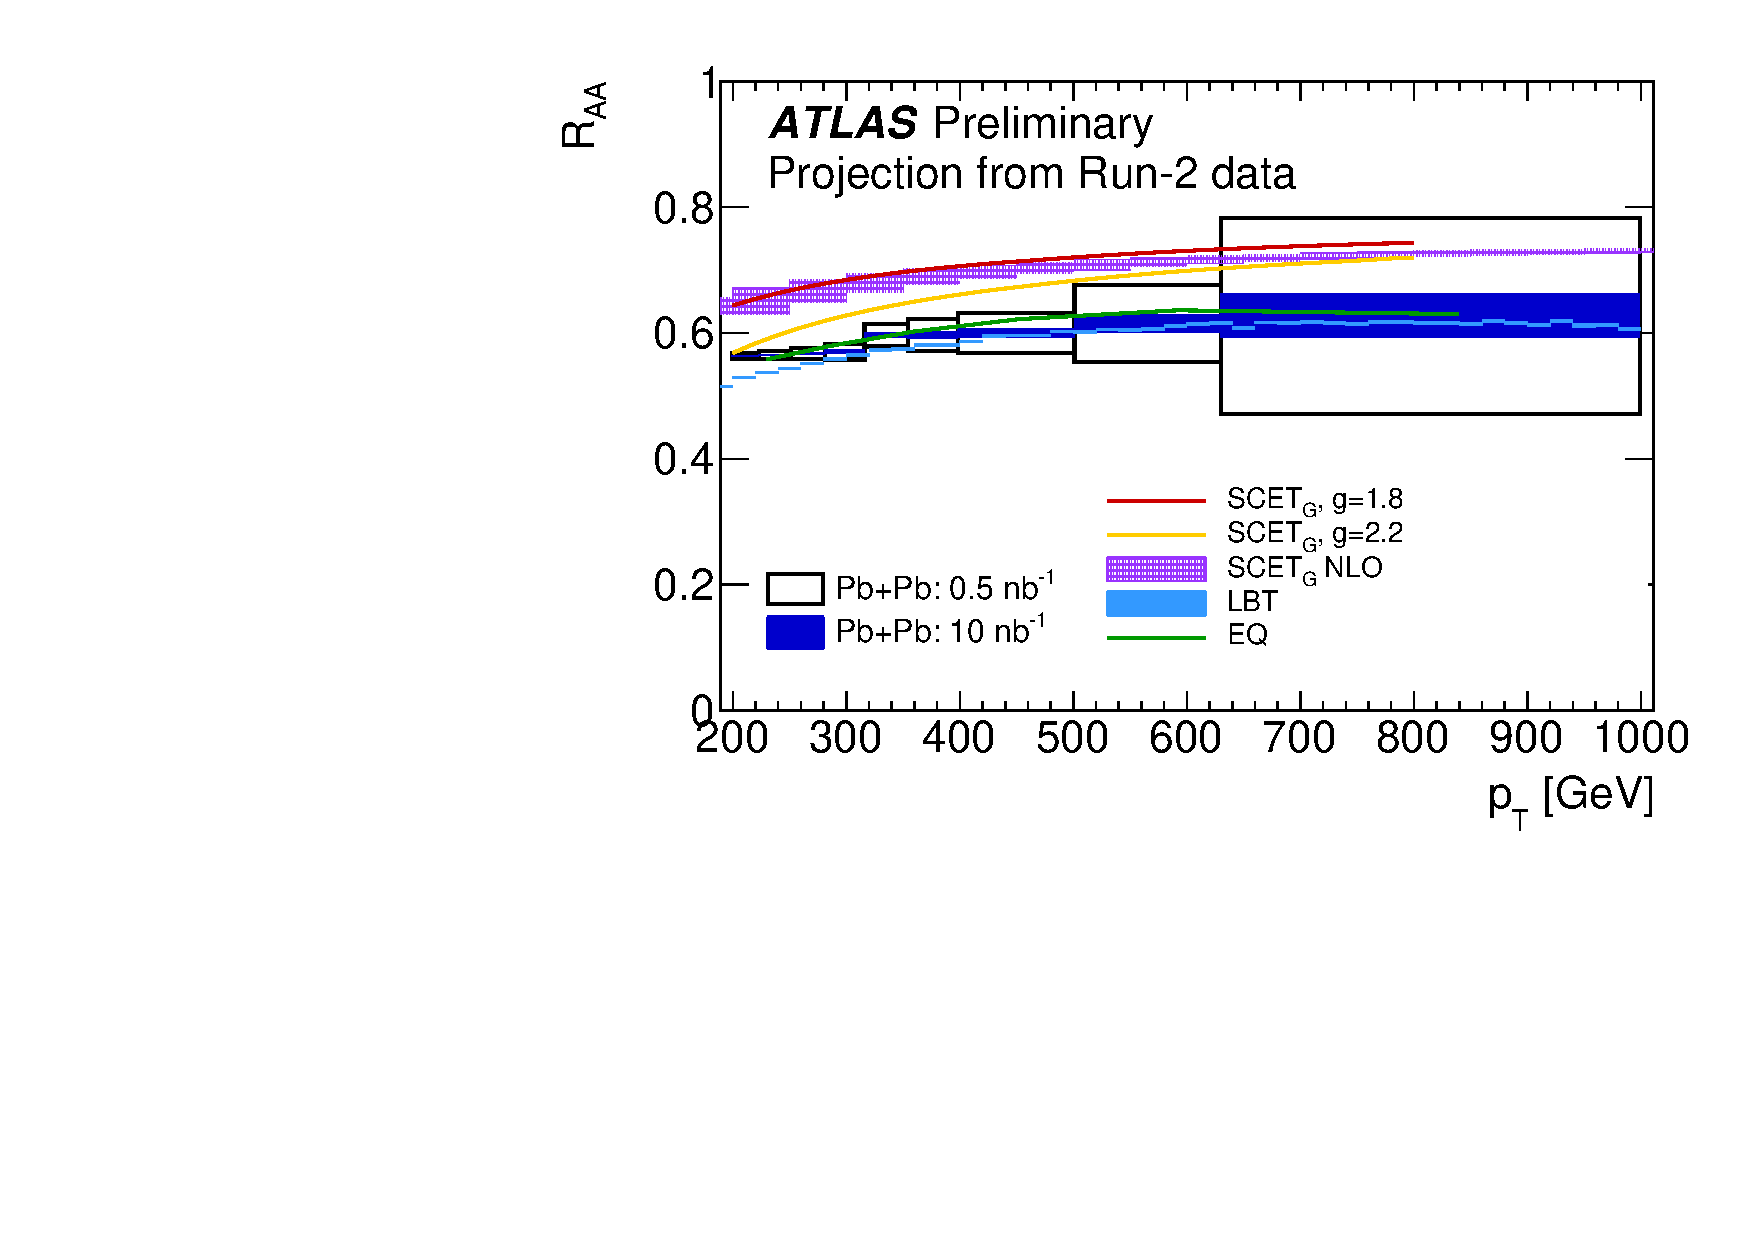
\includegraphics[width=.45\textwidth]{\main/jets/figures/atlas/fig_01a.pdf}
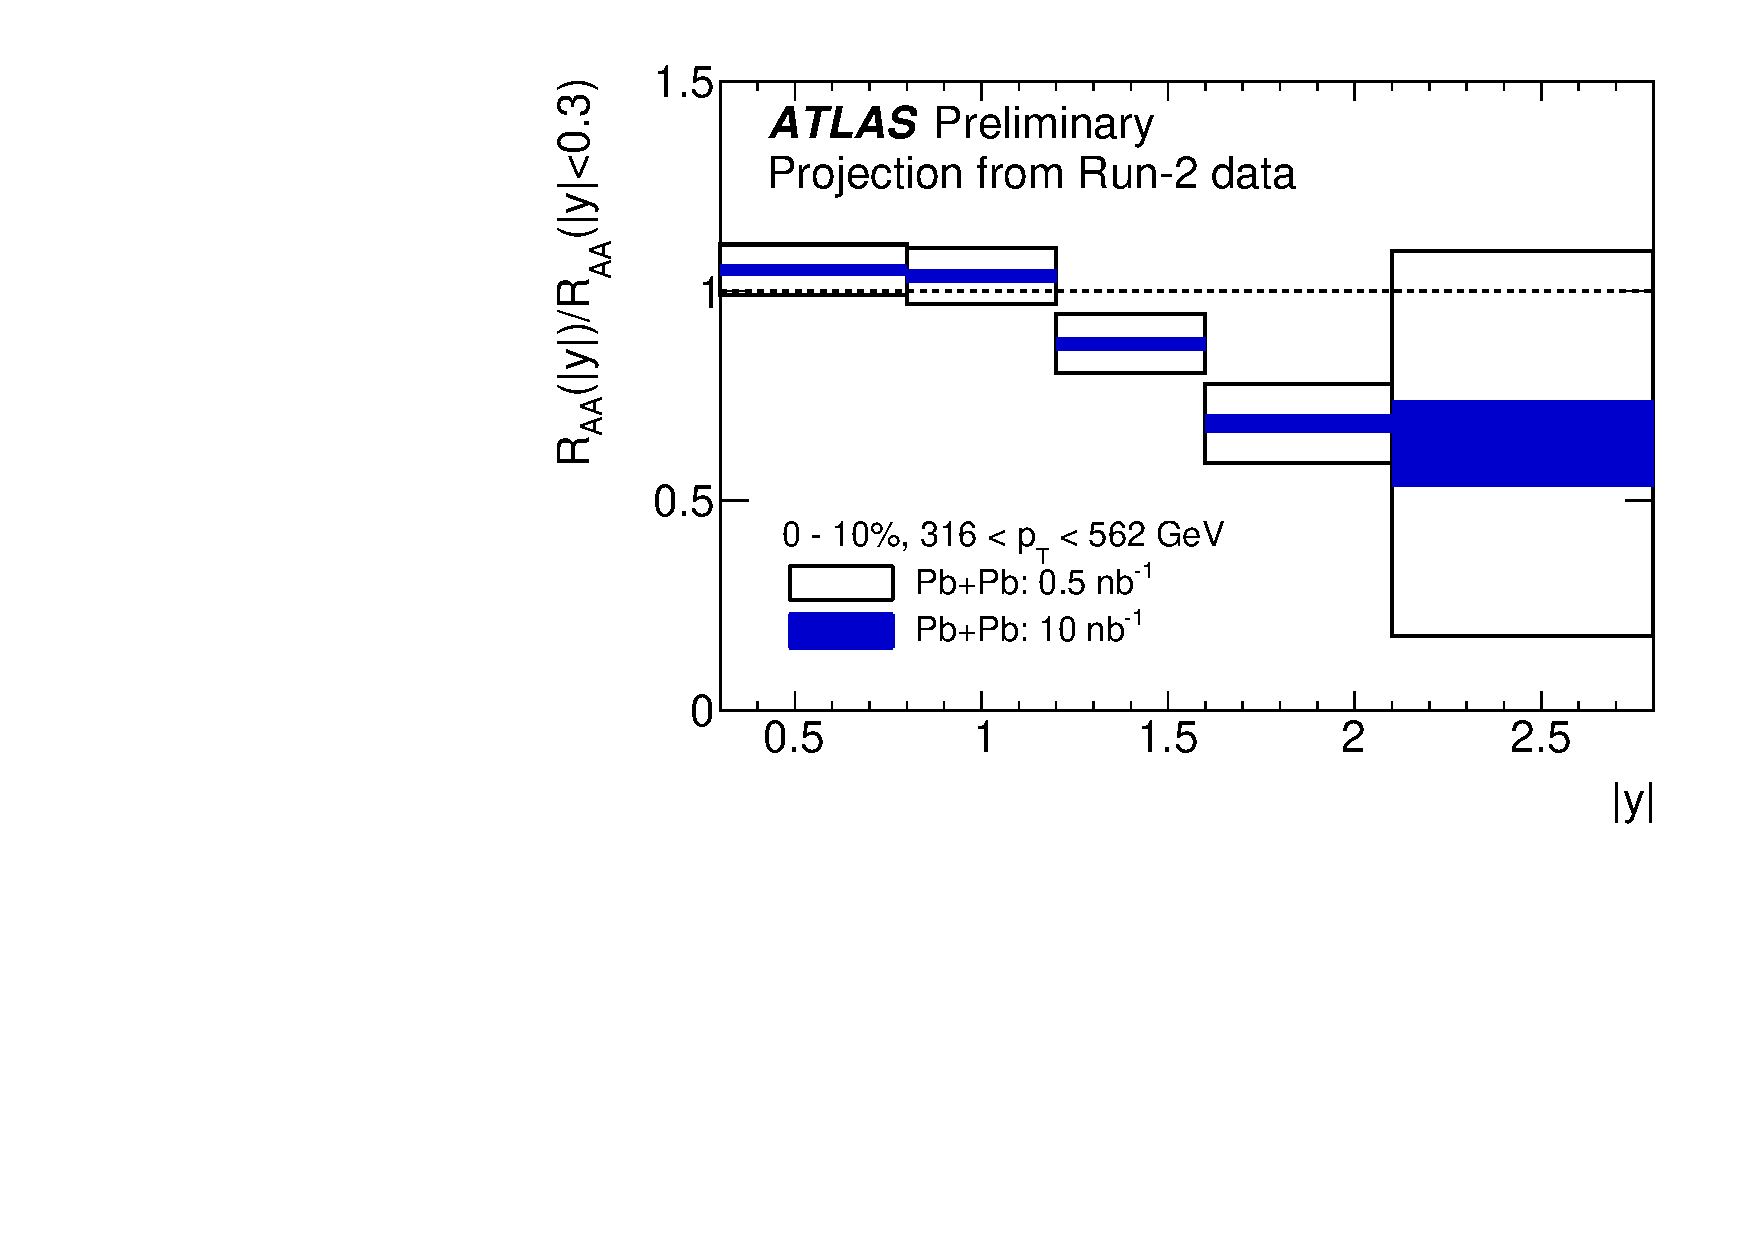
\includegraphics[width=.45\textwidth]{\main/jets/figures/atlas/fig_01b.pdf}
\caption{Projection of the precision that can be reached for jet $R_{\mathrm{AA}}$ at the HL-LHC using calorimeter jets at ATLAS as function of $\pT$ (left panel) and rapidity (right panel)~\cite{ATL-PHYS-PUB-2018-019}. See text for model details.}
\label{fig:jetRAA}
\end{center}
\end{figure}


Parton energy loss can be studied more differentially using boson tagged jets. The bosons (photons or Z$^{0}$ bosons) escape the region of the hot dense medium unmodified. This has been confirmed through the absence of significant modification of both photon and Z$^{0}$ boson production rates in Pb--Pb collisions relative to expectations from measured cross section in pp collisions by both ATLAS and CMS collaborations~\cite{Aad:2012ew,Aad:2015lcb,Chatrchyan:2012vq,Chatrchyan:2014csa}. However, the partons recoiling from the boson is modified in heavy ion collisions due to interactions with the QCD medium. Furthermore, jets produced opposite to the isolated boson
are more likely to originate from quarks, while dijet and hadron+jet correlations usually involve significant gluon contributions. 
Comparing Z+jet and $\gamma$+jet observables to dijets~\cite{Chatrchyan:2011sx,Chatrchyan:2012nia} (or hadron+jets~\cite{Adam:2015doa}) allows to explore the difference between energy loss for quark and gluon initiated jets. Figures~\ref{fig:photonjet} and~\ref{fig:Zjet} show the expected performance at the HL-LHC for the transverse momentum balance between the jet and the boson. The central values are based on the smoothed data from the previous CMS publications~\cite{Sirunyan:2017jic,Sirunyan:2017qhf}. The systematic uncertainties are reduced by a factor of two with respect to the results with the 2015 Pb--Pb data due to improvements on the jet energy scale and jet energy resolution uncertainties available with the larger data sample at the HL-LHC. The collected number of $\gamma$+jet events will also be sufficient to study the path length dependence of jet quenching by performing measurements as a function of angle with the reaction plane for the first time. In addition to the smaller uncertainties due to the enhanced statistics at the HL-LHC, it will also be possible to utilize higher momentum photons and Z$^{0}$ bosons allowing the measurement of larger jet energy losses. The LHC experiments also envision extending the jet momentum reach to lower transverse momentum in certain analyses, allowing to recover those heavily quenched jets which are currently not selected for such measurements due to limitation arising from the fluctuating background. A distinct effect due to large backgrounds is that of limited jet energy resolution, which can be improved by using more sophisticated techniques for the background correction as was recently shown in Ref.~\cite{Haake:2018hqn}.

%the large uncorrelated background jet yield that is not corrected in those approaches. This problem has been addressed generally for coincidence observables by the utilization of statistical correction techniques \cite{Adam:2015doa,Adamczyk:2017yhe}. 

%{\it (pmj Nov 5: note changes to last few sentences of foregoing paragraph. There are two distinct effects due to background: correction for uncorrelated yield, and smearing of jet \pT. These are not the same, and the distinction should be made clearly. From my standpoint the problem due both effects of measuring low \pT{} jets in large background is solved using the statistical correction approach, which should be cited. It remains to show in a publication that this approach works for calorimetric jets, but it is the conceptually correct approach - event-by-event correction for uncorrelated yield can only be approximate even in principle - and there are no show-stoppers as far as I can tell. Some experiments may choose not to use that approach, but that is a choice of approach, not a requirement.)
%(ms Nov 7: I think the low-pt paragraph is fine, even if someone may admit that we should not need Run 3 and 4 to access low-pt stuff for which we should have had enough data already)
}

\begin{figure}[!ht]
\begin{center}
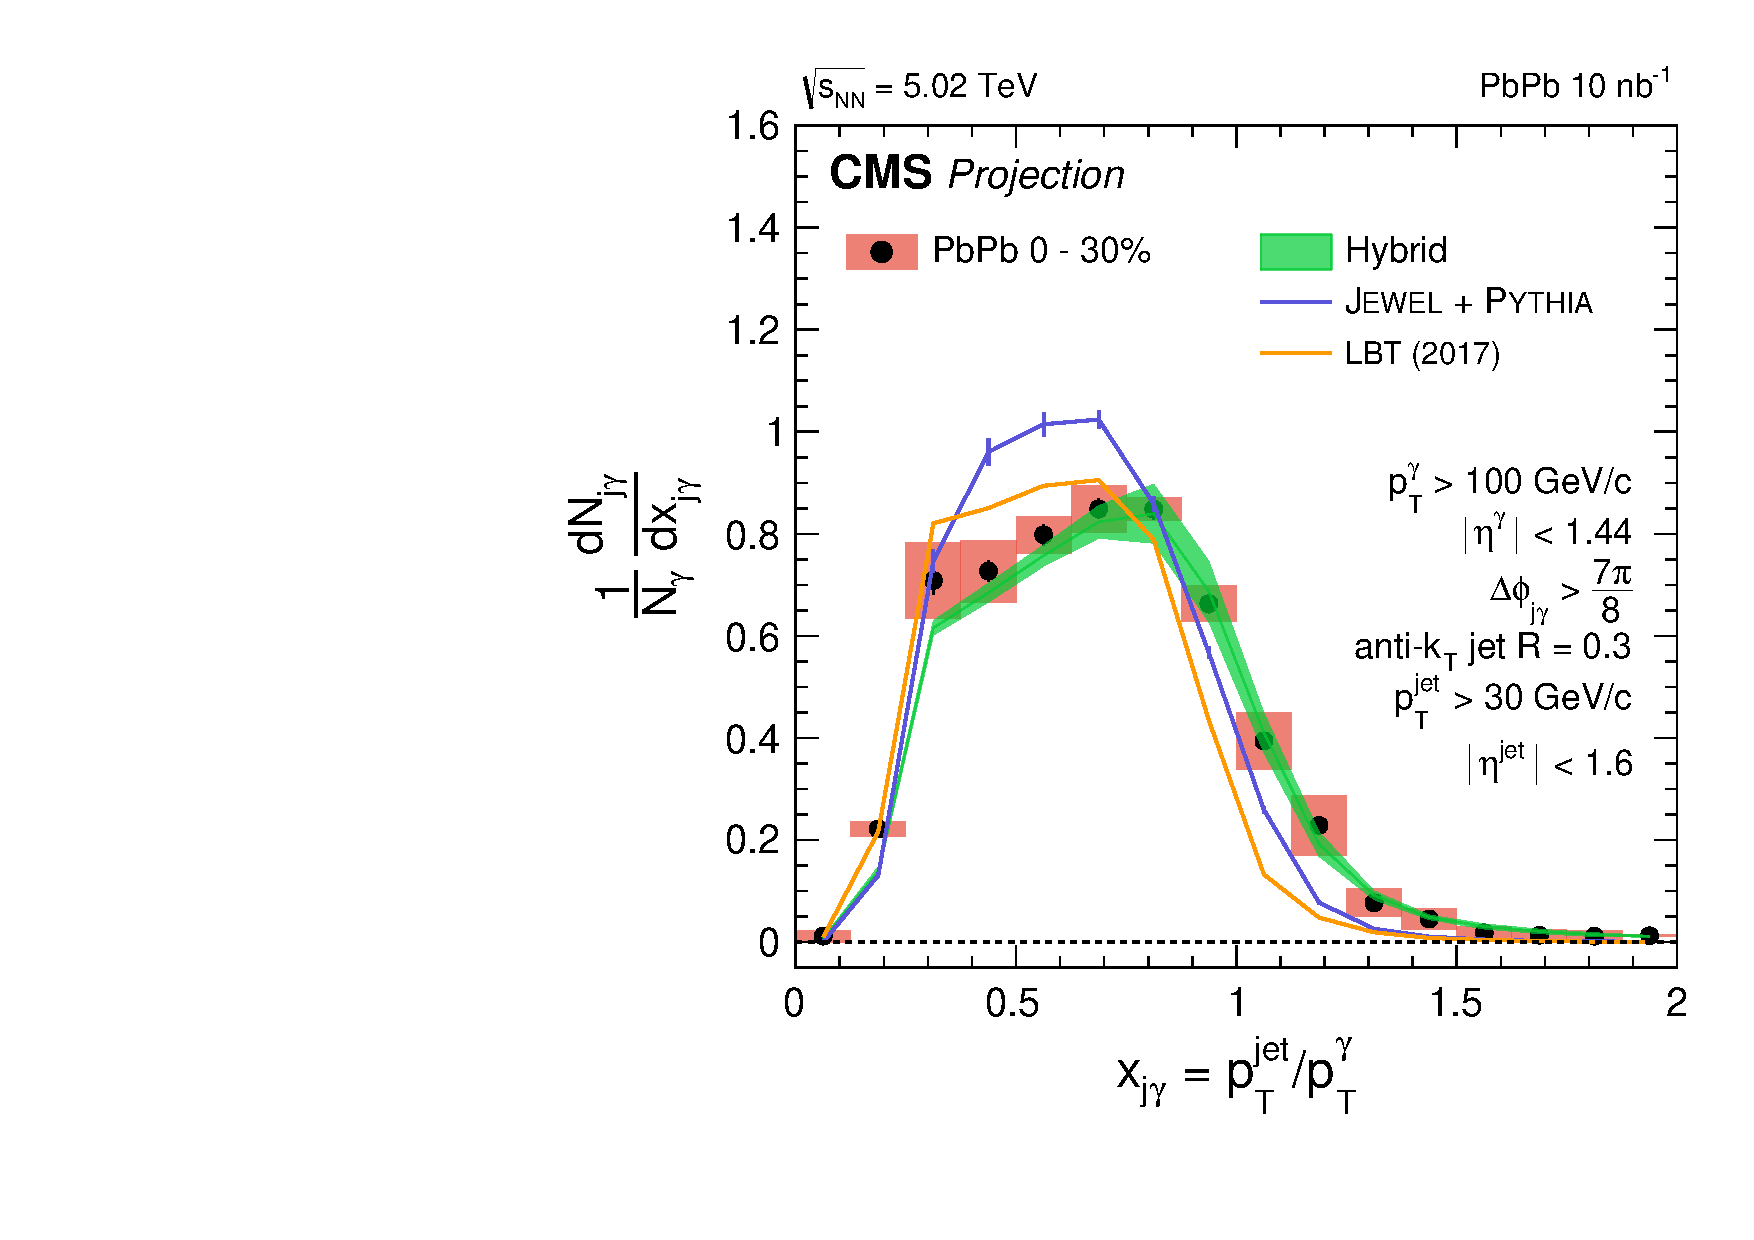
\includegraphics[width=.45\textwidth]{\main/jets/figures/cms/xjg_projection_2.pdf}
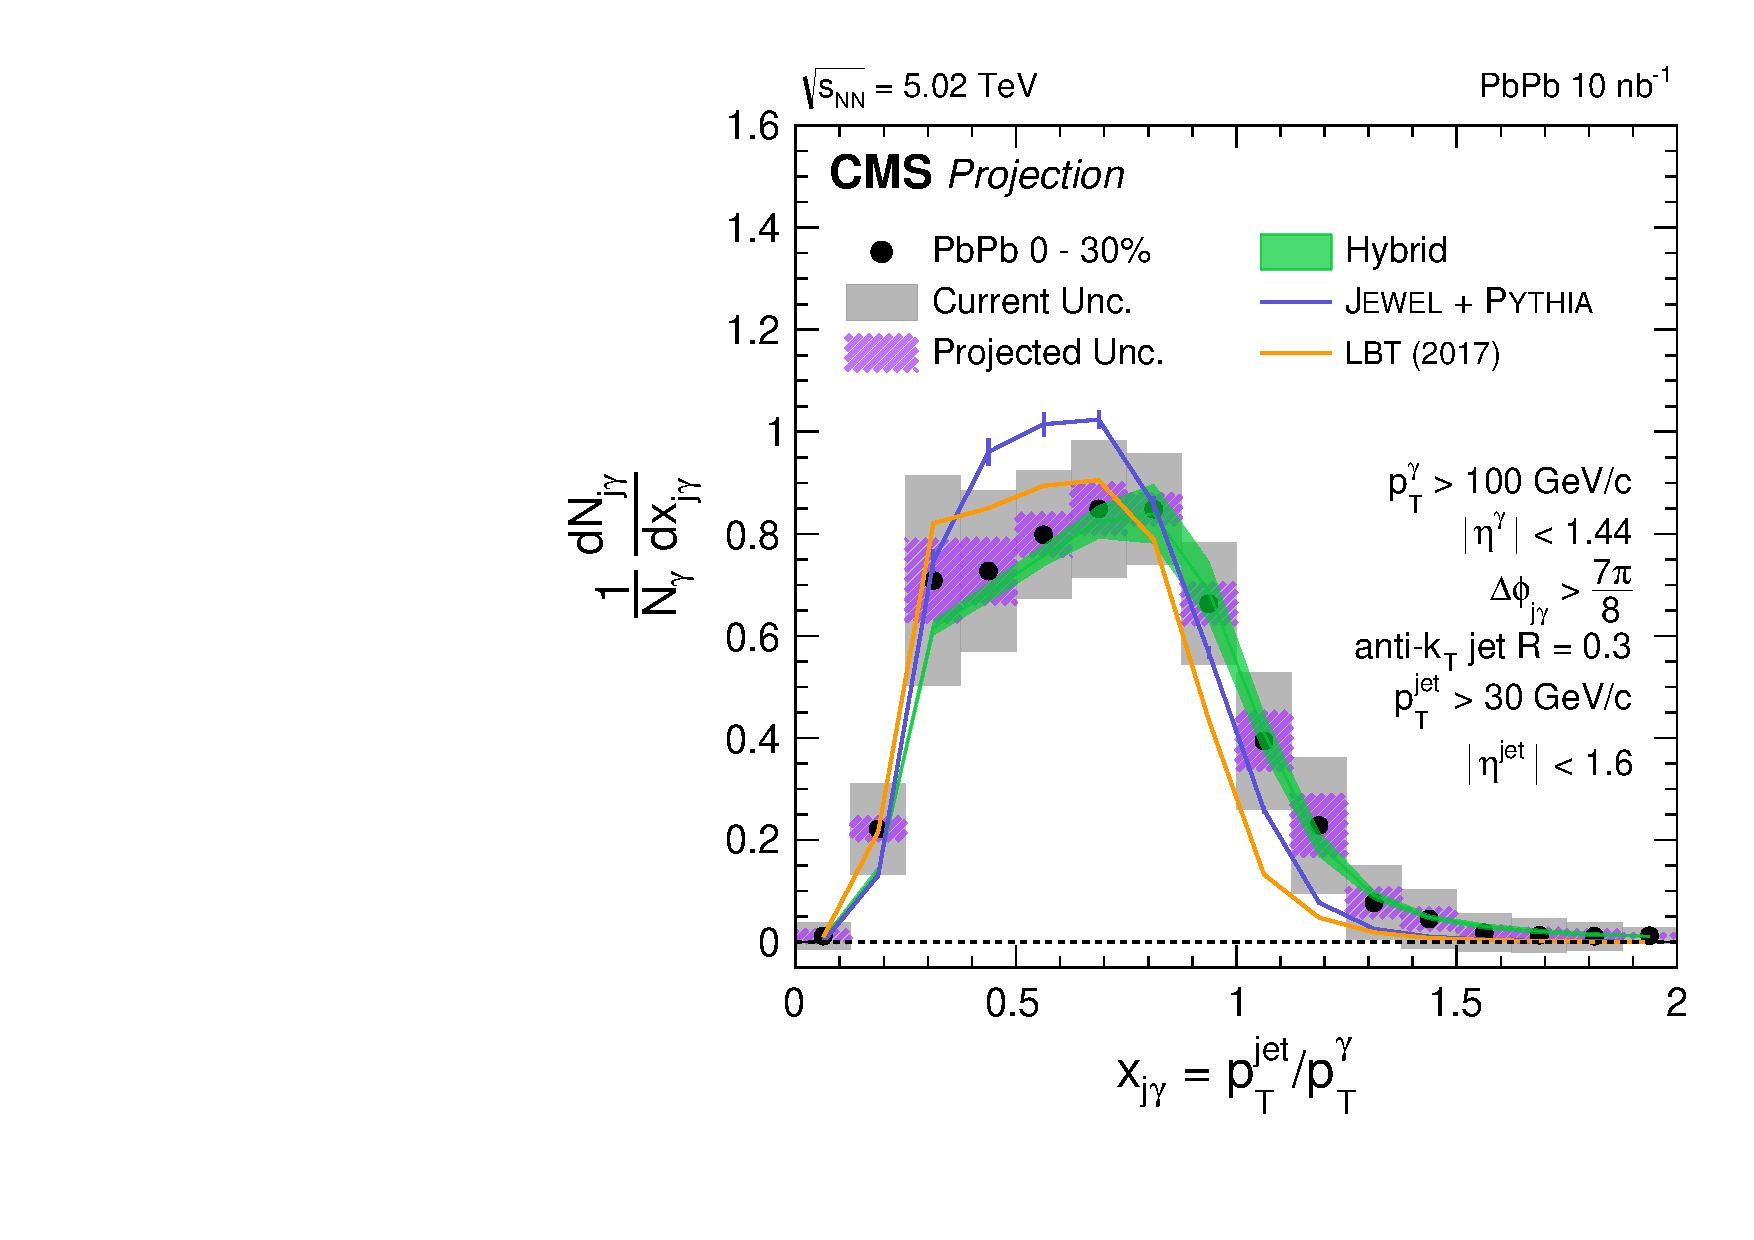
\includegraphics[width=.45\textwidth]{\main/jets/figures/cms/xjg_projection.pdf}
\caption{(Left Panel) Photon-jet momentum balance $x_{j\gamma}$ distribution for isolated-photon+jets of $p_{\gamma}$ $> $ 100 GeV/c and $|\eta_{\gamma}|<1.44$, $p_{\rm jet} > $ 30 GeV/c and $|\eta_{\rm jet}| < 1.6$ in the HL-LHC data (Right Panel). Comparison between the current performance with 0.4 nb$^{-1}$ of Pb--Pb data collected in 2015 and with HL-LHC data~\cite{CMS-FTR-17-002:2017dec}.}
\label{fig:photonjet}
\end{center}
\end{figure}
%
\begin{figure}[!ht]
\begin{center}
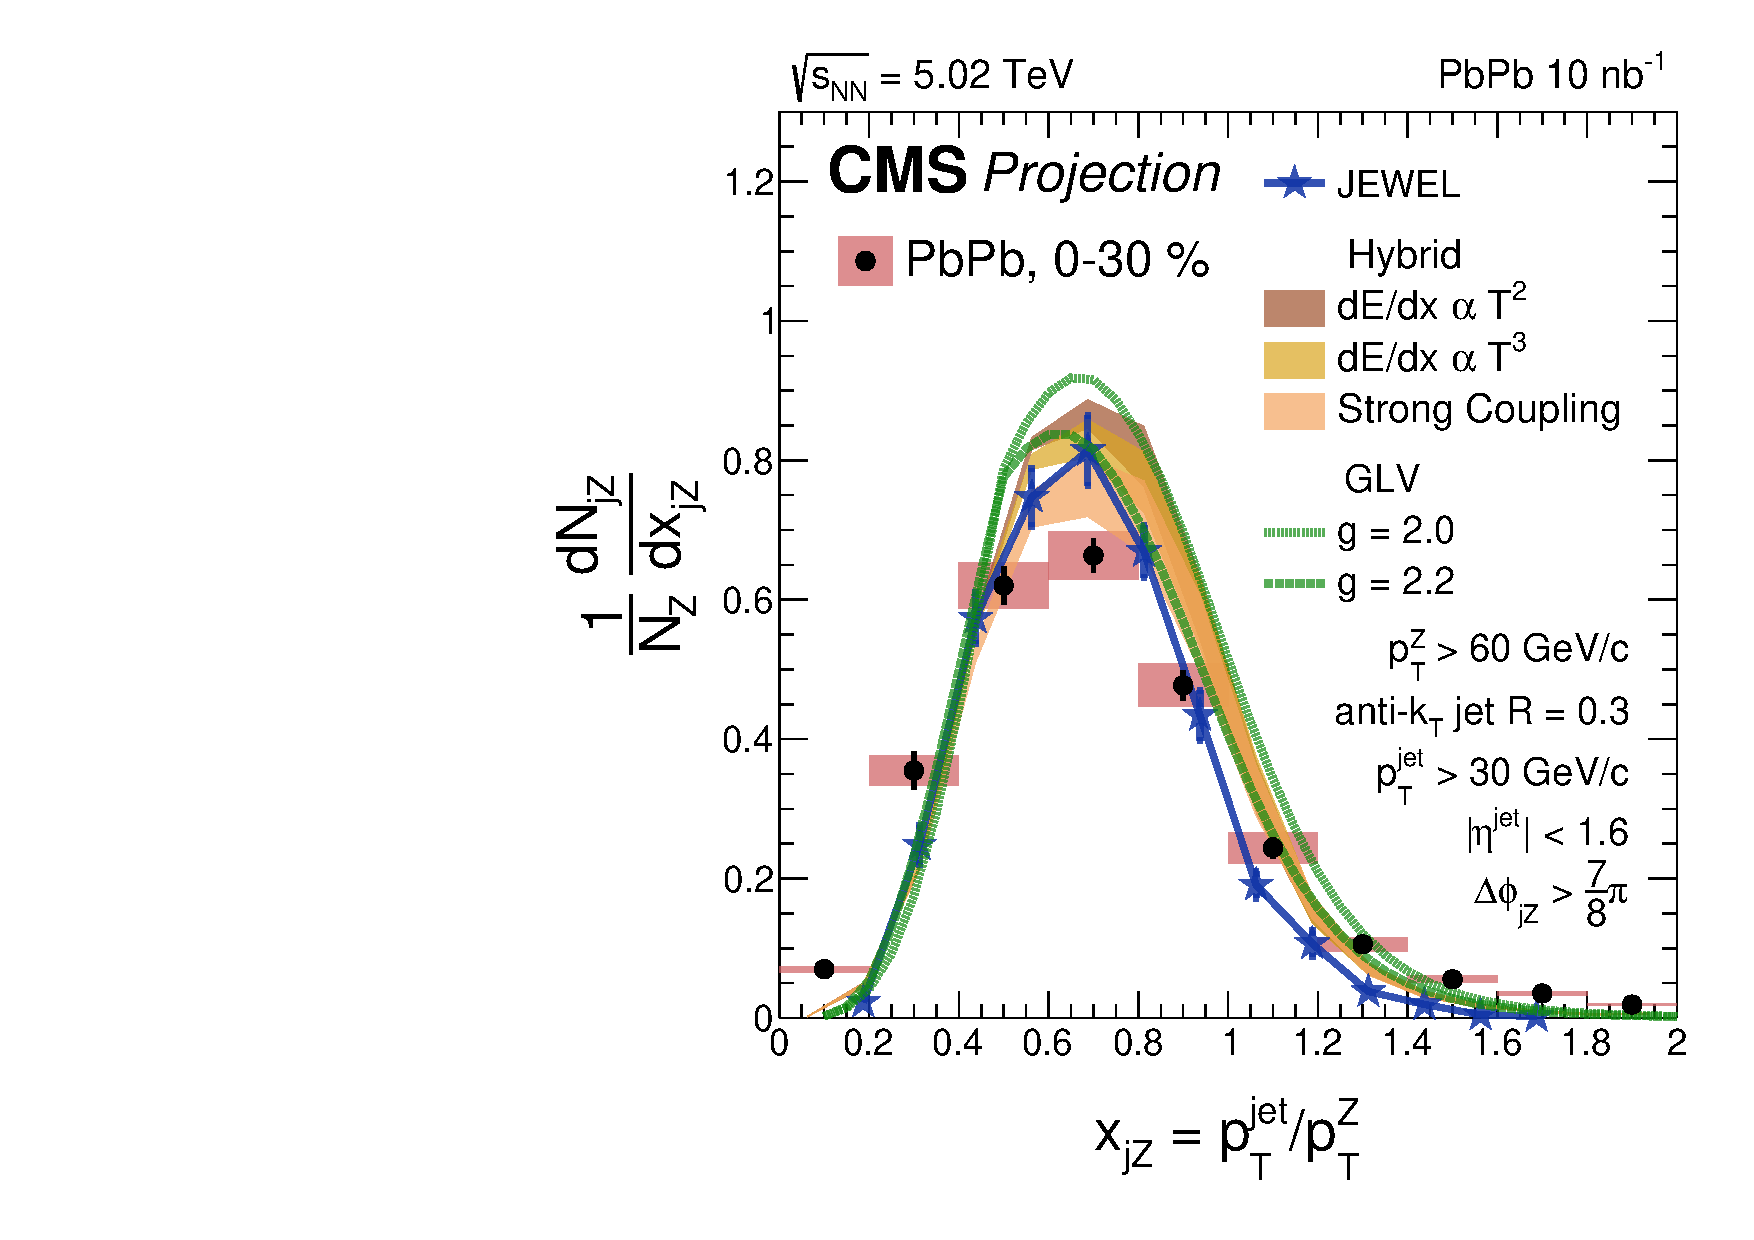
\includegraphics[width=.45\textwidth]{\main/jets/figures/cms/projection_xjz_Theory_sysReduced50Prct.pdf}
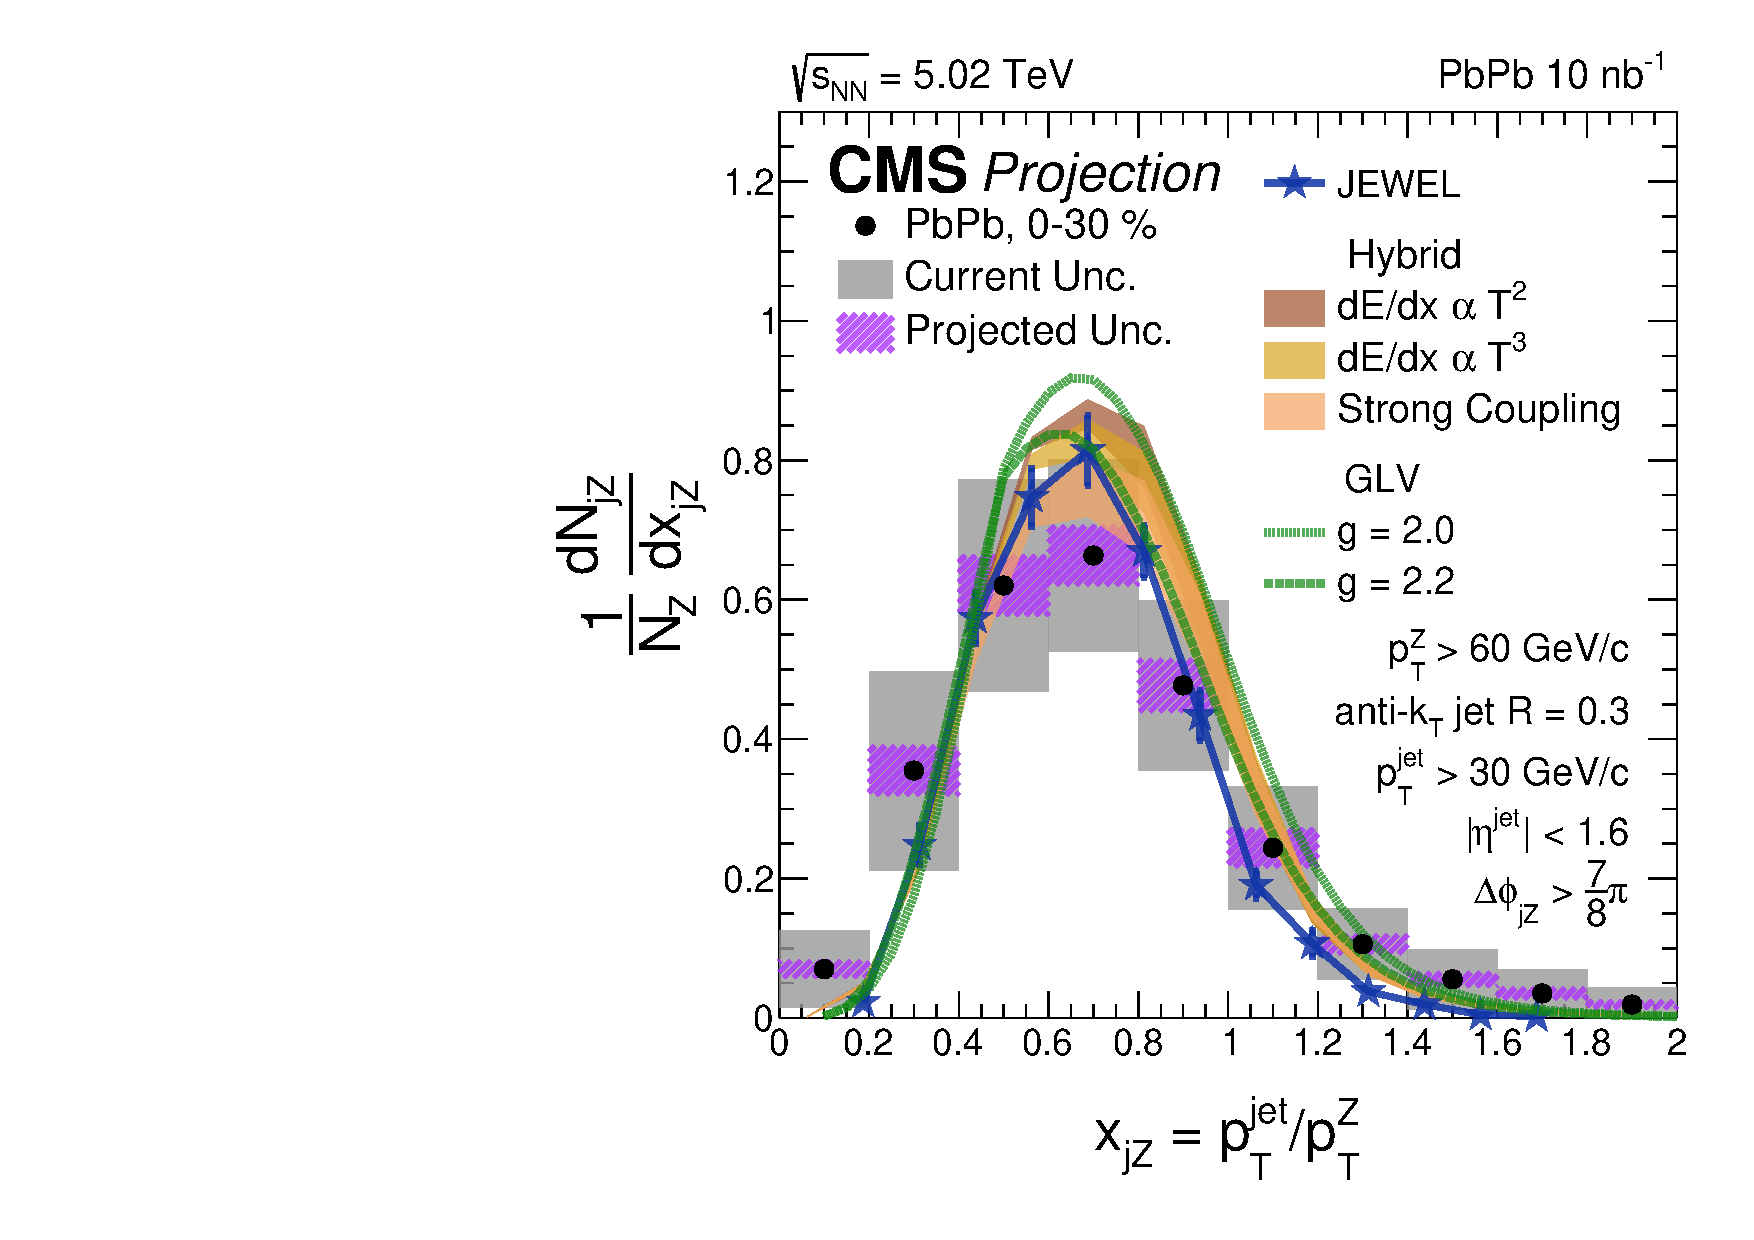
\includegraphics[width=.45\textwidth]{\main/jets/figures/cms/projection_xjz_Theory_MergedUnc_sysReduced50Prct.pdf}
\caption{(Left Panel) $X_{jZ}$ distribution for Z boson-jet pairs with $p_\mathrm{T}^{Z}$ $> $ 60 GeV/c, $p_{\rm jet} > $ 30 GeV/c and $|\eta_{\rm jet}| < 1.6$ in the HL-LHC data (Right Panel) Comparison between the current performance with 0.4 nb$^{-1}$ of Pb--Pb data collected in 2015 and with HL-LHC data~\cite{CMS-FTR-17-002:2017dec}.}
\label{fig:Zjet}
\end{center}
\end{figure}
